\documentclass[12pt]{article}

% Packages
\usepackage[margin=1in]{geometry}
\usepackage{amsmath,amssymb,amsthm}
\usepackage{enumitem}
\usepackage{hyperref}
\usepackage{xcolor}
\usepackage{import}
\usepackage{xifthen}
\usepackage{pdfpages}
\usepackage{transparent}
\usepackage{listings}
\usepackage{tikz}
\usepackage{physics}
\usepackage{siunitx}
\usepackage{booktabs}
\usepackage{cancel}
  \usetikzlibrary{calc,patterns,arrows.meta,decorations.markings}


\DeclareMathOperator{\Log}{Log}
\DeclareMathOperator{\Arg}{Arg}

\lstset{
    breaklines=true,         % Enable line wrapping
    breakatwhitespace=false, % Wrap lines even if there's no whitespace
    basicstyle=\ttfamily,    % Use monospaced font
    frame=single,            % Add a frame around the code
    columns=fullflexible,    % Better handling of variable-width fonts
}

\newcommand{\incfig}[1]{%
    \def\svgwidth{\columnwidth}
    \import{./Figures/}{#1.pdf_tex}
}
\theoremstyle{definition} % This style uses normal (non-italicized) text
\newtheorem{solution}{Solution}
\newtheorem{proposition}{Proposition}
\newtheorem{problem}{Problem}
\newtheorem{lemma}{Lemma}
\newtheorem{theorem}{Theorem}
\newtheorem{remark}{Remark}
\newtheorem{note}{Note}
\newtheorem{definition}{Definition}
\newtheorem{example}{Example}
\newtheorem{corollary}{Corollary}
\theoremstyle{plain} % Restore the default style for other theorem environments
%

% Theorem-like environments
% Title information
\title{Designing a Hands Free Single Stringed Guitar}
\author{Jerich Lee}
\date{\today}

\begin{document}

\maketitle
The lap steel guitar is a stringed instrument that is played while laid horizontally on a
performer’s lap or stand. Pedal actuated tuning systems were introduced to the lap steel guitar,
allowing the performer to quickly change the tune of the strings without interfering with their ability
to perform. However, the additions of such tuning devices increase the price of a lap steel guitar
from hundreds of dollars to thousands. Since a simple lap steel guitar is a low-cost instrument for
musicians and an accessible avenue for hobbyists to build their own guitar, a simple and cheap
mechanism for ergonomically changing the tune of the strings has great potential in the consumer
market. By using the fundamental principles of static analysis, additive manufacturing, and wood
construction, this group has designed a simple, low cost, and accessible pedal actuated prototype
tuning device for a lap steel guitar.

There are a few engineering challenges in creating the mechanism to change the pitch of the
guitar string. The main problem of interest is creating a mechanism under a cost constraint, which
operates with low friction, has ease of manufacturability, and has a straightforward way to install the
mechanism on the body of the guitar. The actuation of the mechanism should be adjustable so that a
wide array of desired tones can be reached. For the mechanism to accurately achieve these tones, the
required change in displacement of the strings needed to reach a final frequency had to be calculated
using static analysis. The force required to change the distance must also be calculated so that the
design of the pedal ensures it can apply a large enough force. Knowing how much force is required
and what force is realistic also provides an upper bound to the range of deformations and changes in
frequencies that are possible using intermediate steps of the pedal. For the sake of this prototype,
the string gauge used is 024. The string will be tuned to an initial frequency of 207.7 Hz or G\#3, and
the prototype mechanism will aim to achieve a final frequency of 220.16 Hz or A3.
The proposed design solution that will be used is a simple rotary spring mechanism. The
mechanism works by using an L-beam structure on each side of the headstock, as shown in Figure 1.

\begin{figure}[htbp]
  \centering
  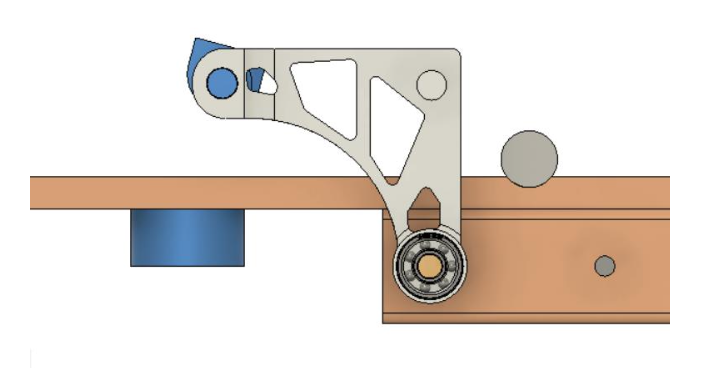
\includegraphics[width=0.8\textwidth]{classes/Mathematics-of-Guitar-Strings/06-10/fgs/fig1.png}
  \caption{L-Beam about Central Axis Point}
  \label{fig:}
\end{figure}

Each L-beam rotates about a central axis point with ball bearings and is connected by a rod.
The mechanism is manufactured in three composite parts for ease of manufacturability and
assembly using Fused Filament Fabrication or 3D printing, as shown in Figure 2.

\begin{figure}[htbp]
  \centering
  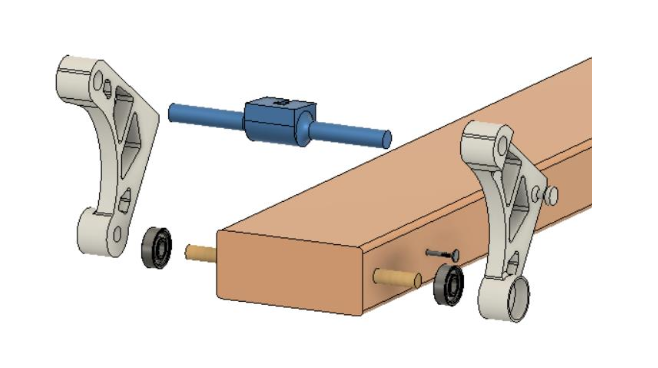
\includegraphics[width=0.8\textwidth]{classes/Mathematics-of-Guitar-Strings/06-10/fgs/fig2.png}
  \caption{Exploded View of Rotary Spring Mechanism}
  \label{fig:}
\end{figure}

Ball bearings are used to ensure minimal friction of the rotary spring mechanism and to
guarantee exact fittings between the body of the guitar and the L-Beams. A ball bearing is press-
fitted into each L-Beam, which goes through a shoulder screw that is screwed into a threaded insert
on each side of the body of the guitar, as shown in Figure 3. A through hole was drilled into the
side of the main guitar body with an 8 mm diameter to accommodate the threaded inserts and
shoulder screws.

\begin{figure}[htbp]
  \centering
  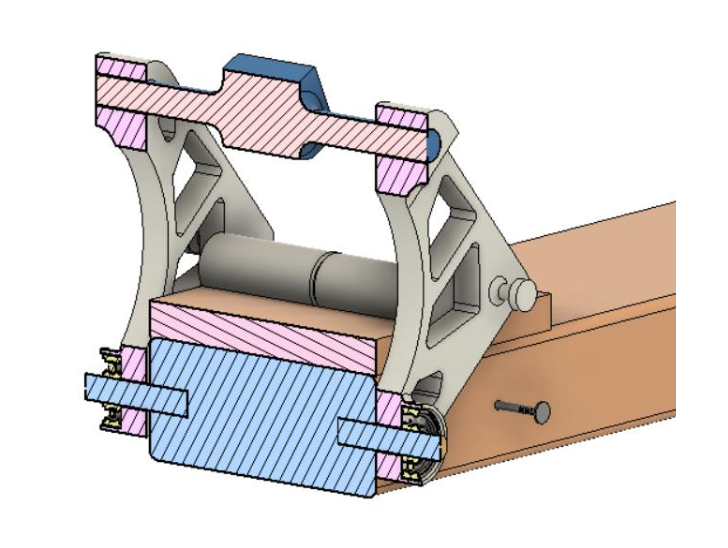
\includegraphics[width=0.8\textwidth]{classes/Mathematics-of-Guitar-Strings/06-10/fgs/fig3.png}
  \caption{Cross-Sectional View of Rotary Spring Mechanism}
  \label{fig:}
\end{figure}

Using a Bowden cable system tethered from a foot pedal to the mechanism, as shown in
Figure 4, the user can quickly transition from an actuated state, as shown in Figure 5, to a rested
state, as shown in Figure 6.

\begin{figure}[htbp]
  \centering
  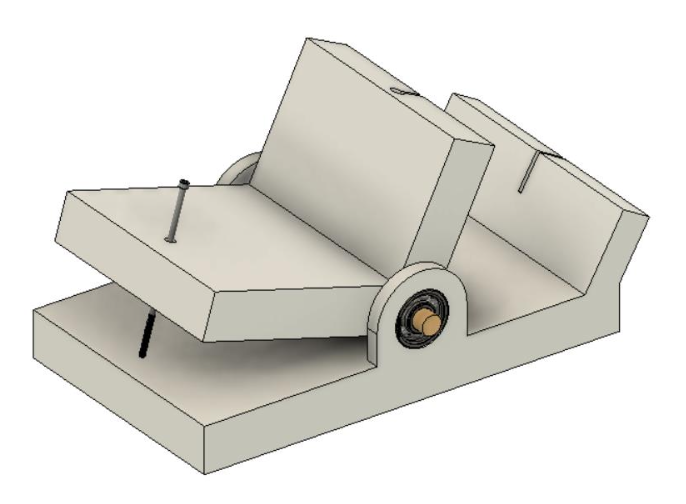
\includegraphics[width=0.8\textwidth]{classes/Mathematics-of-Guitar-Strings/06-10/fgs/fig4.png}
  \caption{Side Angle View of Foot Pedal}
  \label{fig:}
\end{figure}

\begin{figure}[htbp]
  \centering
  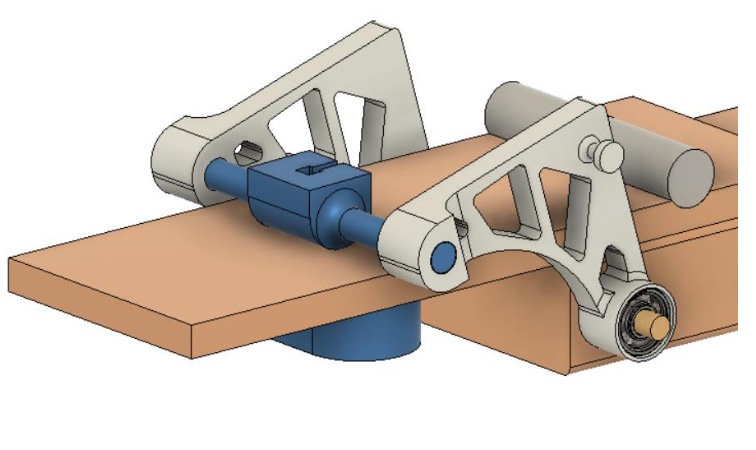
\includegraphics[width=0.8\textwidth]{classes/Mathematics-of-Guitar-Strings/06-10/fgs/fig5.png}
  \caption{Actuated State of Rotary Spring Mechanism}
  \label{fig:}
\end{figure}

\begin{figure}[htbp]
  \centering
  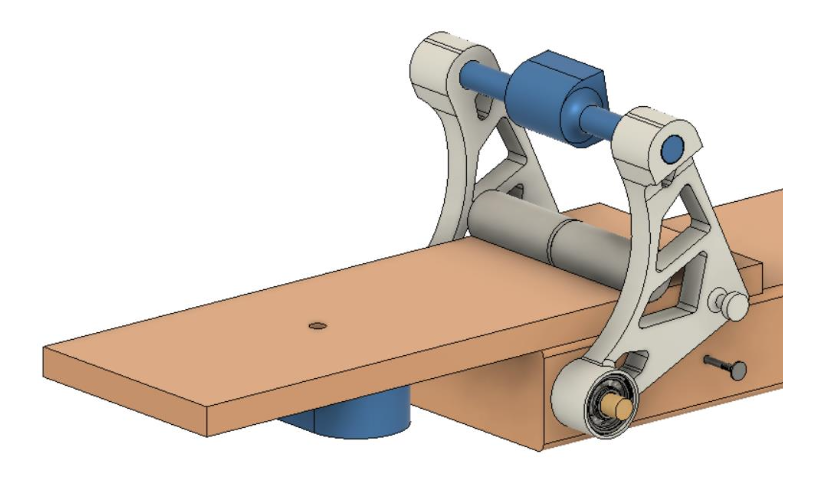
\includegraphics[width=0.8\textwidth]{classes/Mathematics-of-Guitar-Strings/06-10/fgs/fig6.png}
  \caption{Rested State of Rotary Spring Mechanism}
  \label{fig:}
\end{figure}

The tension from the Bowden cable created by force applied by the user through the foot
pedal generates an external moment about the central axis point, which is counteracted by an
opposing moment supplied by loop springs. These loop springs are connected to the main body of
the guitar using screws. The loop springs keep the mechanism tensile, providing controlled motion
and the ability to automatically return the mechanism to the rested state from the actuated state. At
each end of the Bowden cable, there is a ball with a larger diameter than the thickness of the cable.
The Bowden cable is placed securely by using a cable locking system that attaches each end of the
Bowden cable from the pedal to the headstock. The cable locking system was designed to have
pockets that the ball at each end of the Bowden cable can slide into. When the ball ends of the cable
are in these pockets, the balls will catch on the locking system and pull the mechanisms within the
machine when the Bowden cable is actuated. The cable locking system is featured on the rod that
connects the two L-Beams, as shown in Figure 7, and the foot pedal, as shown in Figure 8.

\begin{figure}[htbp]
  \centering
  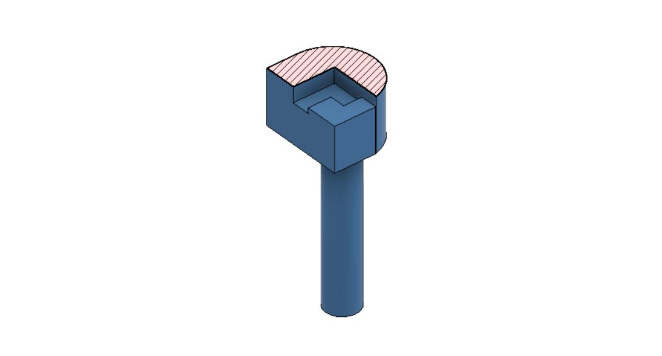
\includegraphics[width=0.8\textwidth]{classes/Mathematics-of-Guitar-Strings/06-10/fgs/fig7.png}
  \caption{Cross-Sectional View of Rod with Cable Locking System}
  \label{fig:}
\end{figure}

\begin{figure}[htbp]
  \centering
  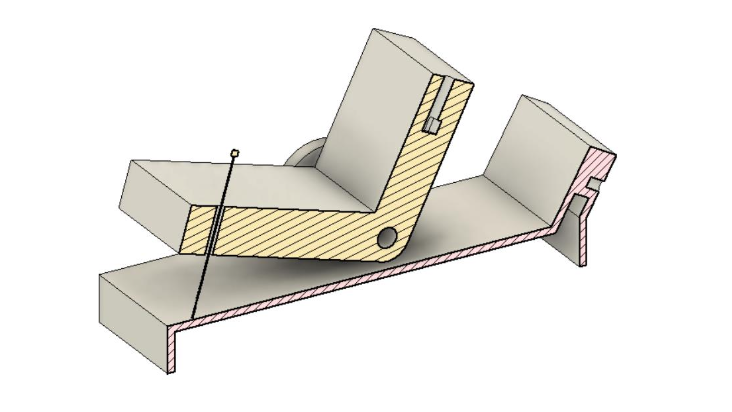
\includegraphics[width=0.8\textwidth]{classes/Mathematics-of-Guitar-Strings/06-10/fgs/fig8.png}
  \caption{Cross-Sectional View of Foot Pedal with Cable Locking System}
  \label{fig:}
\end{figure}

\end{document}
